\section{Kernel debugging}

\begin{frame}[fragile]
  \frametitle{Debugging using messages (1/3)}
  Three APIs are available
  \begin{itemize}
  \item The old \kfunc{printk}, no longer recommended for new debugging
    messages
  \item The \code{pr_*()} family of functions: \kfunc{pr_emerg},
    \kfunc{pr_alert}, \kfunc{pr_crit}, \kfunc{pr_err},
    \kfunc{pr_warn}, \kfunc{pr_notice}, \kfunc{pr_info},
    \kfunc{pr_cont} \\
    and the special \kfunc{pr_debug} (see next pages)
    \begin{itemize}
    \item Defined in \kfile{include/linux/printk.h}
    \item They take a classic format string with arguments
    \item Example:
      \begin{minted}{c}
pr_info("Booting CPU %d\n", cpu);
      \end{minted}
    \item Here's what you get in the kernel log:
      \begin{verbatim}
[  202.350064] Booting CPU 1
      \end{verbatim}
    \end{itemize}
    \item \kfunc{print_hex_dump_debug}: useful to dump a buffer with
      \code{hexdump} like display
  \end{itemize}
\end{frame}

\begin{frame}[fragile]
  \frametitle{Debugging using messages (2/3)}
  \begin{itemize}
  \item The \code{dev_*()} family of functions: \kfunc{dev_emerg},
    \kfunc{dev_alert}, \kfunc{dev_crit}, \kfunc{dev_err},
    \kfunc{dev_warn}, \kfunc{dev_notice}, \kfunc{dev_info} \\
    and the special \kfunc{dev_dbg} (see next page)
    \begin{itemize}
    \item They take a pointer to \kstruct{device} as first
      argument, and then a format string with arguments
    \item Defined in \kfile{include/linux/dev_printk.h}
    \item To be used in drivers integrated with the Linux device
      model
    \item Example:
      \begin{minted}{c}
dev_info(&pdev->dev, "in probe\n");
      \end{minted}
    \item Here's what you get in the kernel log:
      \begin{verbatim}
[   25.878382] serial 48024000.serial: in probe
[   25.884873] serial 481a8000.serial: in probe
      \end{verbatim}
    \end{itemize}
  \item \code{*_ratelimited()} version exists which limits the amount of print
    if called too much based on \code{/proc/sys/kernel/printk_ratelimit{_burst}}
    values
  \end{itemize}
\end{frame}

\begin{frame}[fragile]
  \frametitle{Debugging using messages (3/3)}
  \begin{itemize}
  \item The kernel defines many more format specifiers than the standard
    \code{printf()} existing ones.
  \begin{itemize}
    % \path of package url directly supports percent characters, unless it is
    % used inside arguments of other macros which is the case of the \code macro
    \item {\codecolor \path{%p}}: Display the hashed value of pointer by default.
    \item {\codecolor \path{%px}}: Always display the address of a pointer (use
      carefully on non-sensitive addresses).
    \item {\codecolor \path{%pK}}: Display hashed pointer value, zeros or the
      pointer address depending on \code{kptr_restrict} sysctl value.
    \item {\codecolor \path{%pOF}}: Device-tree node format specifier.
    \item {\codecolor \path{%pr}}: Resource structure format specifier.
    \item {\codecolor \path{%pa}}: Physical address display (work on all architectures 32/64
      bits)
    \item {\codecolor \path{%pe}}: Error pointer (displays the string
      corresponding to the error number)
  \end{itemize}
  \item \code{/proc/sys/kernel/kptr_restrict} should be set to \code{1} in order
    to display pointers using {\codecolor \path{%pK}}
  \item See \kdochtml{core-api/printk-formats} for an exhaustive list of supported format
    specifiers
  \end{itemize}
\end{frame}

\begin{frame}
  \frametitle{pr\_debug() and dev\_dbg()}
  \begin{itemize}
  \item When the driver is compiled with \code{DEBUG} defined, all
    these messages are compiled and printed at the debug level.
    \code{DEBUG} can be defined by \codewithhash{\#define DEBUG} at the
    beginning of the driver, or using
    \code{ccflags-$(CONFIG_DRIVER) += -DDEBUG} in the \code{Makefile}
  \item When the kernel is compiled with \kconfig{CONFIG_DYNAMIC_DEBUG},
    then these messages can dynamically be enabled on a per-file,
    per-module or per-message basis, by writing commands to
    \code{/proc/dynamic_debug/control}. Note that messages are not enabled
    by default.
    \begin{itemize}
    \item Details in \kdochtml{admin-guide/dynamic-debug-howto}
    \item Very powerful feature to only get the debug messages you're
      interested in.
    \end{itemize}
  \item When neither \code{DEBUG} nor \kconfig{CONFIG_DYNAMIC_DEBUG} are
    used, these messages are not compiled in.
  \end{itemize}
\end{frame}

\ifthenelse{\equal{\training}{debugging}}{
\begin{frame}
  \frametitle{pr\_debug() and dev\_dbg() usage}
  \begin{itemize}
  \item Debug prints can be enabled using the
    \code{/proc/dynamic_debug/control} file.
  \begin{itemize}
    \item \code{cat /proc/dynamic_debug/control} will display all
      lines that can be enabled in the kernel
    \item Example: \code{init/main.c:1427 [main]run_init_process =p "    \%s\012"}
  \end{itemize}
  \item A syntax allows to enable individual print using lines, files or modules
  \begin{itemize}
    \item \code{echo "file drivers/pinctrl/core.c +p" > /proc/dynamic_debug/control}
      will enable all debug prints in \code{drivers/pinctrl/core.c}
    \item \code{echo "module pciehp +p" > /proc/dynamic_debug/control}
      will enable the debug print located in the \code{pciehp} module
    \item \code{echo "file init/main.c line 1427 +p" > /proc/dynamic_debug/control}
      will enable the debug print located at line 1247 of file \code{init/main.c}
    \item Replace \code{+p} with \code{-p} to disable the debug print
  \end{itemize}
  \end{itemize}
\end{frame}
}{}

\ifthenelse{\equal{\training}{linux-kernel}}{
\begin{frame}
  \frametitle{Configuring the priority}
  \begin{itemize}
  \item Each message is associated to a priority, ranging from \code{0} for
    emergency to \code{7} for debug, as specified in
    \kfile{include/linux/kern_levels.h}.
  \item All the messages, regardless of their priority, are stored in
    the kernel log ring buffer
    \begin{itemize}
    \item Typically accessed using the \code{dmesg} command
    \end{itemize}
  \item Some of the messages may appear on the console, depending on
    their priority and the configuration of
    \begin{itemize}
    \item The \code{loglevel} kernel parameter, which defines the
      priority number below which messages are displayed on the console.
      Details in \kdochtml{admin-guide/kernel-parameters}.
      \newline Examples: \code{loglevel=0}: no message, \code{loglevel=8}: all messages
    \item The value of \code{/proc/sys/kernel/printk}, which allows to
      change at runtime the priority above which messages are
      displayed on the console. Details in
      \kdochtml{admin-guide/sysctl/kernel}
    \end{itemize}
  \end{itemize}
\end{frame}
}{}

\ifthenelse{\equal{\training}{debugging}}{
\begin{frame}
  \frametitle{Debug logs troubleshooting}
  \begin{itemize}
    \item When using dynamic debug, make sure that your debug call is enabled: it must be visible in
    \code{control} file in debugfs \textbf{and} be activated (\code{=p})
    \item Is your log output only in the kernel log buffer?
    \begin{itemize}
      \item You can see it thanks to \code{dmesg}
      \item You can lower the \code{loglevel} to output it to  the console directly
      \item You can also set \code{ignore_loglevel} in the kernel command line to
      force all kernel logs to console
    \end{itemize}
    \item If you are working on an out-of-tree module, you may prefer to define \code{DEBUG} in
    your module source or Makefile instead of using dynamic debug
    \item If configuration is done through the kernel command line, is it
    properly interpreted?
    \begin{itemize}
      \item Starting from 5.14, kernel will let you know about faulty
      command line:\\
      \code{Unknown kernel command line parameters loglevel, will be passed to user
      space.}
      \item You may need to take care of special characters escaping (e.g: quotes)
    \end{itemize}
    \item Be aware that a few subsystems bring their own logging infrastructure, with specific
    configuration/controls, eg: \code{drm.debug=0x1ff}
  \end{itemize}
\end{frame}
}{}


\begin{frame}
  \frametitle{DebugFS}
  A virtual filesystem to export debugging information to user space.
  \begin{itemize}
  \item Kernel configuration: \kconfig{CONFIG_DEBUG_FS}
    \begin{itemize}
    \item \code{Kernel hacking -> Debug Filesystem}
    \end{itemize}
  \item The debugging interface disappears when Debugfs is
    configured out.
  \item You can mount it as follows:
    \begin{itemize}
    \item \code{sudo mount -t debugfs none /sys/kernel/debug}
    \end{itemize}
  \item First described on \url{https://lwn.net/Articles/115405/}
  \item API documented in the Linux Kernel Filesystem API:
    \kdochtml{filesystems/debugfs}
    {The debugfs filesystem}
  \end{itemize}
\end{frame}

\begin{frame}[fragile]
  \frametitle{DebugFS API}
  \begin{itemize}
  \item Create a sub-directory for your driver:
    \begin{minted}{c}
struct dentry *debugfs_create_dir(const char *name,
                                  struct dentry *parent);
    \end{minted}
  \item Expose an integer as a file in DebugFS. Example:
    \begin{minted}{c}
struct dentry *debugfs_create_u8(const char *name, mode_t mode,
                struct dentry *parent, u8 *value);
    \end{minted}
    \begin{itemize}
    \item \code{u8}, \code{u16}, \code{u32}, \code{u64} for decimal representation
    \item \code{x8}, \code{x16}, \code{x32}, \code{x64} for hexadecimal representation
    \end{itemize}
  \item Expose a binary blob as a file in DebugFS:
    \begin{minted}{c}
struct dentry *debugfs_create_blob(const char *name,
                mode_t mode, struct dentry *parent,
                struct debugfs_blob_wrapper *blob);
    \end{minted}

  \item Also possible to support writable DebugFS files or customize
    the output using the more generic \kfunc{debugfs_create_file}
    function.
  \end{itemize}
\end{frame}

\begin{frame}[fragile]
  \frametitle{Using Magic SysRq}
  Functionnality provided by serial drivers
  \begin{itemize}
  \item Allows to run multiple debug / rescue commands even when the
    kernel seems to be in deep trouble
    \begin{itemize}
    \item On PC: press \code{[Alt]} + \code{[Prnt Scrn]} + \code{<character>}
	  simultaneously\\
          (\code{[SysRq]} = \code{[Alt]} + \code{[Prnt Scrn]})
    \item On embedded: in the console, send a break character\\
      (Picocom: press \code{[Ctrl]} + \code{a} followed by \code{[Ctrl]}
      + \code{\ }), then press \code{<character>}
    \end{itemize}
  \item Example commands:
    \begin{itemize}
    \item \code{h}: show available commands
    \item \code{s}: sync all mounted filesystems
    \item \code{b}: reboot the system
    \item \code{n}: makes RT processes nice-able.
    \item \code{w}: shows the kernel stack of all sleeping processes
    \item \code{t}: shows the kernel stack of all running processes
    \item You can even register your own!
    \end{itemize}
  \item Detailed in \kdochtml{admin-guide/sysrq}
  \end{itemize}
\end{frame}


\begin{frame}
  \frametitle{kgdb - A kernel debugger}
  \begin{itemize}
  \item \kconfig{CONFIG_KGDB} in {\em Kernel hacking}.
  \item The execution of the kernel is fully controlled by \code{gdb}
    from another machine, connected through a serial line.
  \item Can do almost everything, including inserting breakpoints in
    interrupt handlers.
  \item Feature supported for the most popular CPU architectures
  \item \kconfig{CONFIG_GDB_SCRIPTS} allows to build GDB python scripts that are
    provided by the kernel.
  \begin{itemize}
	  \item See \kdochtml{process/debugging/kgdb} for more information
  \end{itemize}
  \end{itemize}
\end{frame}

\ifthenelse{\equal{\training}{debugging}}{

\begin{frame}
  \frametitle{kgdb kernel config}
  \begin{itemize}
    \item \kconfigval{CONFIG_DEBUG_KERNEL}{y} to make KGDB support visible
    \item \kconfigval{CONFIG_KGDB}{y} to enable KGDB support
    \item \kconfigval{CONFIG_DEBUG_INFO}{y} to compile the kernel with debug info (\code{-g})
    \item \kconfigval{CONFIG_FRAME_POINTER}{y} to have more reliable
          stacktraces
    \item \kconfigval{CONFIG_KGDB_SERIAL_CONSOLE}{y} to enable KGDB support
          over serial
    \item \kconfigval{CONFIG_GDB_SCRIPTS}{y} to enable kernel GDB python
          scripts
    \item \kconfigval{CONFIG_RANDOMIZE_BASE}{n} to disable KASLR
    \item \kconfigval{CONFIG_WATCHDOG}{n} to disable watchdog
    \item \kconfigval{CONFIG_MAGIC_SYSRQ}{y} to enable Magic SysReq support
    \item \kconfigval{CONFIG_STRICT_KERNEL_RWX}{n} to disable memory protection
          on code section, thus allowing to put breakpoints
  \end{itemize}
\end{frame}

\begin{frame}
  \frametitle{kgdb pitfalls}
  \begin{itemize}
    \item KASLR should be disabled to avoid confusing gdb with randomized kernel
          addresses
    \begin{itemize}
      \item Disable \em{kaslr} mode using \code{nokaslr} command line parameter
            if enabled in your kernel.
    \end{itemize}
    \item Disable the platform watchdog to avoid rebooting while debugging.
    \begin{itemize}
      \item When interrupted by KGDB, all interrupts are disabled thus, the
            watchdog is not serviced.
      \item Sometimes, watchdog is enabled by upper boot levels. Make sure to
            disable the watchdog there too.
    \end{itemize}
    \item Can not interrupt kernel execution from gdb using \code{interrupt}
          command or \code{Ctrl + C}.
    \item Not possible to break everywhere (see \kconfig{CONFIG_KGDB_HONOUR_BLOCKLIST}).
    \item Need a console driver with polling support.
    \item Some architecture lacks functionalities (No watchpoints on arm32 for
          instance) and some instabilities might happen!
  \end{itemize}
\end{frame}
}{}

\begin{frame}
  \frametitle{Using kgdb (1/2)}
  \begin{itemize}
  \item Details available in the kernel documentation:
    \kdochtml{process/debugging/kgdb}
  \item You must include a kgdb I/O driver. One of them is \code{kgdb} over
    serial console (\code{kgdboc}: \code{kgdb} over console, enabled by
    \kconfig{CONFIG_KGDB_SERIAL_CONSOLE})
  \item Configure \code{kgdboc} at boot time by passing to the kernel:
    \begin{itemize}
    \item \code{kgdboc=<tty-device>,<bauds>}.
    \item For example: \code{kgdboc=ttyS0,115200}
    \end{itemize}
  \item Or at runtime using sysfs:
   \begin{itemize}
   \item \code{echo ttyS0 > /sys/module/kgdboc/parameters/kgdboc}
   \item If the console does not have polling support, this command will yield
         an error.
   \end{itemize}
  \end{itemize}
\end{frame}

\begin{frame}
  \frametitle{Using kgdb (2/2)}
  \begin{itemize}
  \item Then also pass \code{kgdbwait} to the kernel: it makes
    \code{kgdb} wait for a debugger connection.
  \item Boot your kernel, and when the console is initialized,
    interrupt the kernel with a break character and then \code{g}
    in the serial console (see our {\em Magic SysRq} explanations).
  \item On your workstation, start \code{gdb} as follows:
    \begin{itemize}
    \item \code{arm-linux-gdb ./vmlinux}
    \item \code{(gdb) set remotebaud 115200}
    \item \code{(gdb) target remote /dev/ttyS0}
    \end{itemize}
  \item Once connected, you can debug a kernel the way you would debug
    an application program.
  \item On GDB side, the first threads represent the CPU context (ShadowCPU<x>),
    then all the other threads represents a task.
  \end{itemize}
\end{frame}


\begin{frame}
  \frametitle{Debugging with a JTAG interface}
  Two types of JTAG dongles
  \begin{itemize}
  \item The ones offering a \code{gdb} compatible interface, over a
    serial port or an Ethernet connection. \code{gdb} can directly
    connect to them.
  \item The ones not offering a gdb compatible interface are generally
    supported by OpenOCD (Open On Chip Debugger):
    \url{https://openocd.sourceforge.net/}
    \begin{itemize}
    \item OpenOCD is the bridge between the gdb debugging language
      and the JTAG interface of the target CPU.
    \item See the very complete documentation:
      \url{https://openocd.org/pages/documentation.html}
    \item For each board, you'll need an OpenOCD configuration file
      (ask your supplier)
    \end{itemize}
  \end{itemize}
   \begin{center}
     \includegraphics[width=\textwidth]{slides/kernel-driver-development-debugging/jtag.pdf}
   \end{center}
\end{frame}

\begin{frame}
  \frametitle{Early traces}
  \begin{itemize}
  \item If something breaks before the \code{tty} layer, serial driver
    and serial console are properly registered, you might just have
    nothing else after "\code{Starting kernel...}"
  \item On ARM, if your platform implements it, you can activate
    (\kconfig{CONFIG_DEBUG_LL} and \kconfig{CONFIG_EARLY_PRINTK}), and add
    \code{earlyprintk} to the kernel command line
    \begin{itemize}
    \item Assembly routines to just push a character and wait for it to
      be sent
    \item Extremely basic, but is part of the uncompressed section, so
      available even if the kernel does not uncompress correctly!
    \end{itemize}
  \item On other platforms, hoping that your serial driver implements
    \kfunc{OF_EARLYCON_DECLARE}, you can enable \kconfig{CONFIG_SERIAL_EARLYCON}
    \begin{itemize}
    \item The kernel will try to hook an appropriate \code{earlycon}
      UART driver using the \code{stdout-path} of the device-tree.
    \end{itemize}
  \end{itemize}
\end{frame}

\begin{frame}
  \frametitle{More kernel debugging tips 1/2}
  \begin{itemize}
  \item Make sure \kconfig{CONFIG_KALLSYMS_ALL} is enabled
    \begin{itemize}
    \item To get oops messages with symbol names instead of raw
      addresses
    \item Turned on by default
    \end{itemize}
  \item Make sure \kconfig{CONFIG_DEBUG_INFO} is also enabled
    \begin{itemize}
    \item This way, the kernel is compiled with \code{$(CROSSCOMPILE)gcc
        -g}, which keeps the source code inside the binaries.
    \end{itemize}
  \item If your device is not probed, try enabling
        \kconfig{CONFIG_DEBUG_DRIVER}
    \begin{itemize}
    \item Extremely verbose!
    \item Will enable all the debug logs in the device-driver core
      section
    \end{itemize}
  \end{itemize}
\end{frame}

\begin{frame}[fragile]
  \frametitle{More kernel debugging tips 2/2}
  Device Tree output can be better understood with the in-tree \code{dtx_diff} script
  \begin{itemize}
  \item Show the origin of each property/node: \code{scripts/dtc/dtx_diff -T <dts>}
    \begin{minted}[fontsize=\scriptsize]{yaml}
main_i2c3: i2c@20030000 { /* arch/arm64/boot/dts/ti/k3-am62-main.dtsi:450:26-460:4,
                             arch/arm64/boot/dts/ti/k3-am625-beagleplay.dts:820:12-825:3,
                             arch/arm64/boot/dts/ti/k3-am625-beagleplay-custom.dts:20:12-25:3 */
     ...
     reg = <0x00 0x20030000 0x00 0x100>; /* arch/arm64/boot/dts/ti/k3-am62-main.dtsi:452:3-452:38 */
     status = "okay"; /* arch/arm64/boot/dts/ti/k3-am625-beagleplay.dts:824:2-824:18 */

     joystick@52 { /* arch/arm64/boot/dts/ti/k3-am625-beagleplay-custom.dts:21:14-24:4 */
         compatible = "nintendo,nunchuk"; /* arch/arm64/boot/dts/ti/k3-am625-beagleplay-custom.dts:23:3-23:35 */
         reg = <0x52>; /* arch/arm64/boot/dts/ti/k3-am625-beagleplay-custom.dts:22:3-22:16 */
     };
};
    \end{minted}
  \item Can also be used to diff DTS
  \end{itemize}
\end{frame}

\begin{frame}
  \frametitle{Getting help and reporting bugs}
  \begin{itemize}
  \item If you are using a custom kernel from a hardware vendor, contact
        that company. The community will have less interest supporting
        a custom kernel.
  \item Otherwise, or if this doesn't work, try to reproduce the
        issue on the latest version of the kernel.
  \item Make sure you investigate the issue as much as you can: see
    \kdochtml{admin-guide/bug-bisect}
  \item Check for previous bugs reports. Use web search engines,
    accessing public mailing list archives.
  \item If you're the first to face the issue, it's very useful for
    others to report it, even if you cannot investigate it further.
  \item If the subsystem you report a bug on has a mailing list, use
    it. Otherwise, contact the official maintainer (see the
    \kfile{MAINTAINERS} file). Always give as many useful details as
    possible.
  \end{itemize}
\end{frame}

\begin{frame}{Debugging resources}
  \begin{columns}
    \column{0.7\textwidth}
    Checkout Bootlin's debugging training!
    \begin{itemize}
    \item Linux debugging, profiling, tracing and performance analysis training
    \item \url{https://bootlin.com/doc/training/debugging/}
    \item \href{https://bootlin.com/doc/training/debugging/debugging-slides.pdf}{Slides}
      and
      \href{https://bootlin.com/doc/training/debugging/debugging-labs.pdf}{labs}
      are available for free
    \end{itemize}
    \column{0.3\textwidth}
    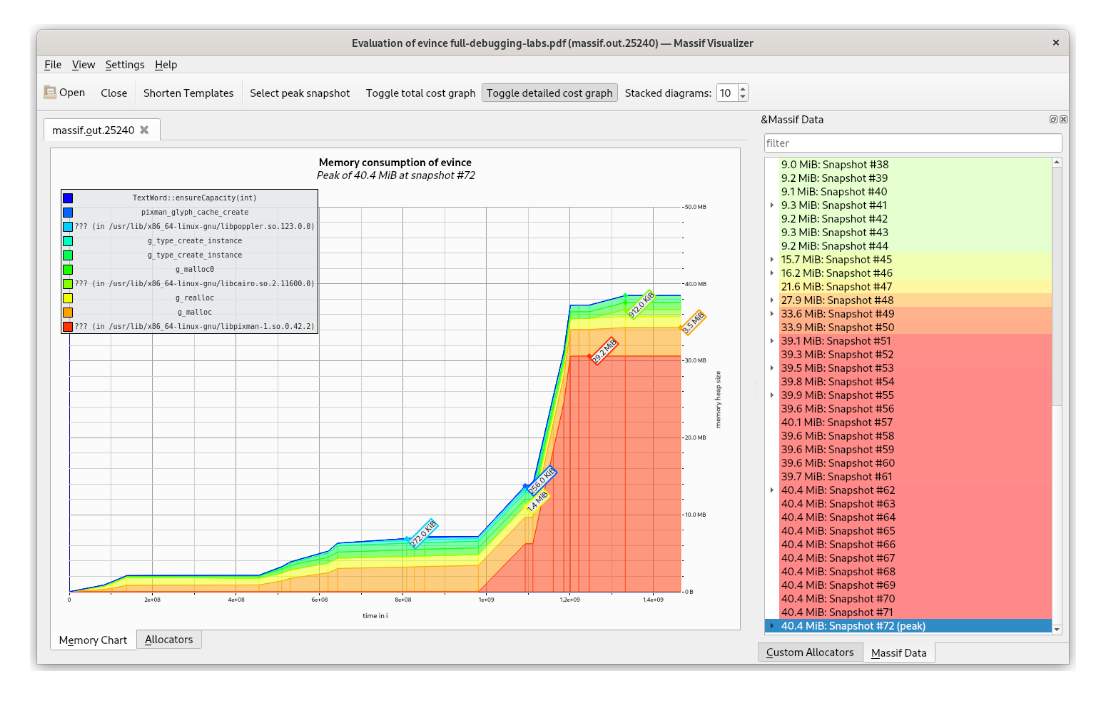
\includegraphics[width=1\textwidth]{slides/kernel-driver-development-debugging/debugging-screenshot.png}
  \end{columns}
\end{frame}

\setuplabframe
{Kernel debugging}
{
  \begin{itemize}
  \item Use the dynamic debug feature.
  \item Add debugfs entries
  \item Load a broken driver and see it crash
  \item Analyze the error information dumped by the kernel.
  \item Disassemble the code and locate the exact C instruction which
    caused the failure.
  \end{itemize}
}
